%------------------------------------------------------------------------
% Chapter:  GUI
%------------------------------------------------------------------------

\chapter{Graphical users interface \label{gui}}

The program {\it PDFFIT Gui} is simply an interface for the pair
distribution function (PDF) refinement program {\it PDFFIT}. This
interface program is part of the {\it DISCUS} program package. {\it
PDFFIT Gui} is intended to provide a simple interface for refining
PDFs without having to know the details of the command language of
the program {\it PDFFIT}. \par

%------------------------------------------------------------------------
\section{Main window}

\begin{figure}[!b]
   \centering
   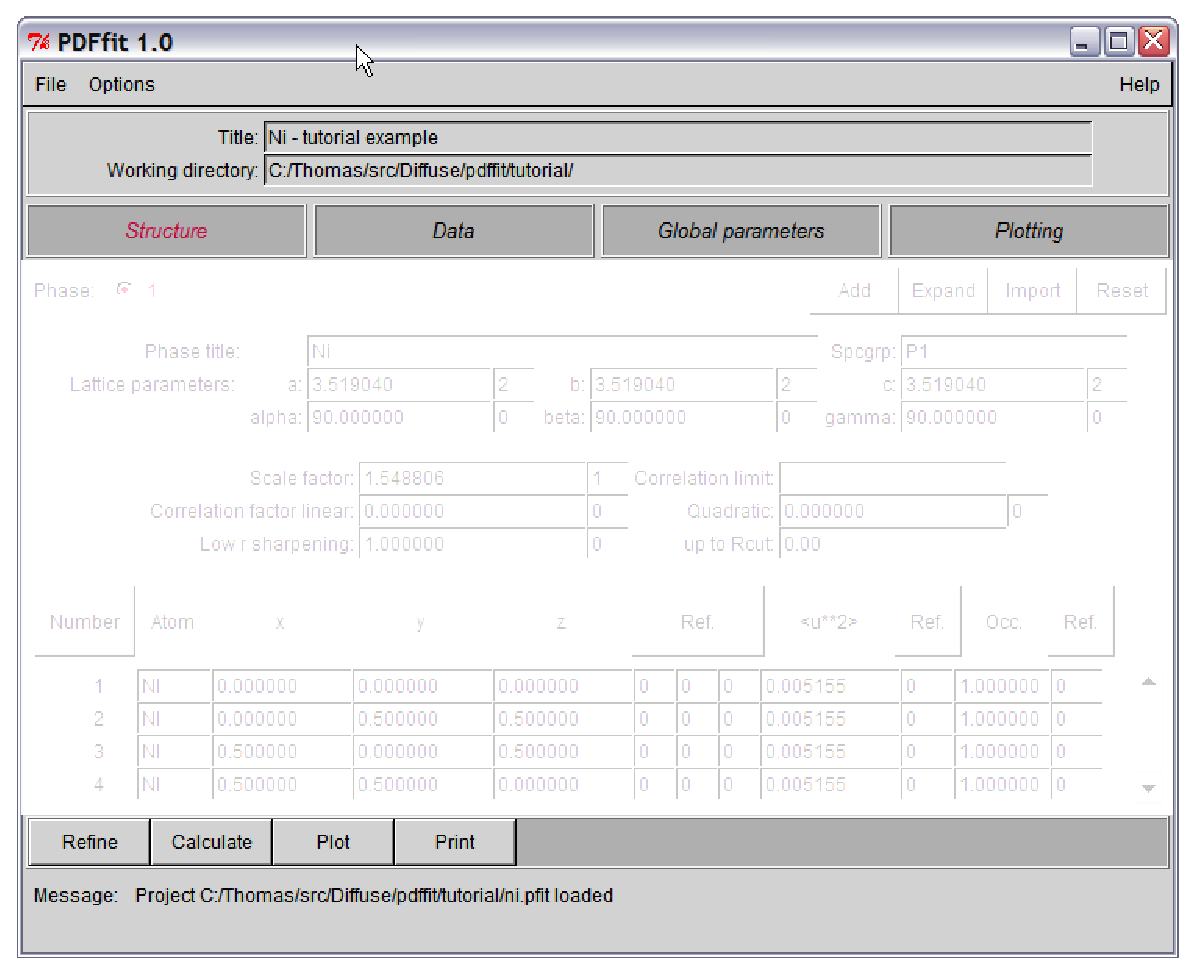
\includegraphics[width=3.5in, angle=0]{use-1.eps}
   \caption{Main window controls of {\it PDFFIT Gui}.}
   \label{fig_use1}
\end{figure}

Figure \ref{fig_use1} shows the graphical interface of the program.
The hidden middle section can show different input areas, that are
discussed in the following sections. Starting from the top, the menu
{\tt File} allows one to load and save complete {\it PDFFIT Gui}
project files as well as exit from the program. The {\tt Options}
menu allows one to customize colors in the graphical interface as
well as the plotting window. \par

Going down, we find input fields for an overall title as well as for
the working directory. Please note, that even under the Windows
operating system, the '/' slash is used in directory names. Going
down further, we see a row of buttons labeled \textbf{Structure},
\textbf{Data}, \textbf{Global parameters} and \textbf{Plotting}.
Clicking these buttons will show the corresponding input area which
are discussed in detail in the following sections. Skipping over
this middle section, we find a row of four buttons at the bottom of
the window:

\begin{itemize}
  \item \textbf{Refine}: This starts the refinement. The middle
  section is automatically changed to show the output of {\it
  PDFFIT}.

  \item \textbf{Calculate}: This will only calculate the PDF from
  the current structural model, but not refine. This feature is
  useful to see the PDF of the initial model or to calculate the PDF
  over a different range in $r$ after a refinement.

  \item \textbf{Plot}: This will plot the experimental PDF as well
  as the model PDF and a difference curve.

  \item \textbf{Print}: This will print or save the current plot.
\end{itemize}

\noindent Finally just below these buttons is the message area used
to output program information as well as warning and error messages.

%------------------------------------------------------------------------
\section{Structure window}

\begin{figure}[!t]
   \centering
   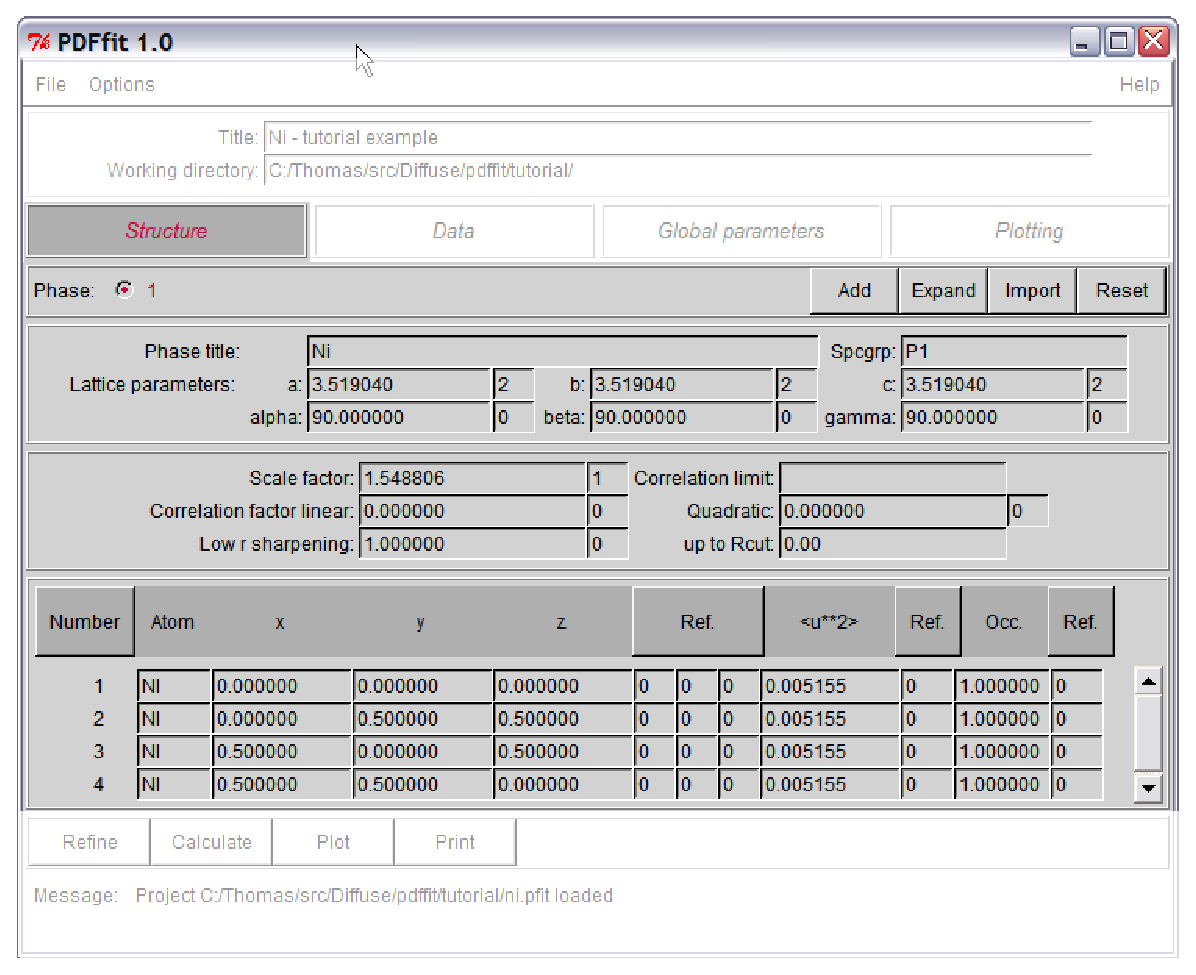
\includegraphics[width=3.5in, angle=0]{use-2.eps}
   \caption{Structure window of {\it PDFFIT Gui}.}
   \label{fig_use2}
\end{figure}

The structure window (as the name suggests) allows the input of all
structure information. Starting from the top in Figure
\ref{fig_use2}, we find a set of radio buttons to select the
structural phase, in our case only one. On the right, there is a set
of four buttons:

\begin{itemize}
  \item \textbf{Add}: This button will add a new phase to the
  project. If the maximum number of phases of the program {\it
  PDFFIT} is exceeded, an error message is shown.

  \item \textbf{Expand}: This command allows one to create all
  symmetrically equivalent atoms from the content of the asymmetric
  unit. Simple enter the lattice parameters, space group and atoms
  of the asymmetric unit and then click this button. As a result,
  {\it all} atoms in the unit cell will be show. Please note, the
  {\it PDFFIT} does not apply any symmetry operations, so the model
  must contain {\it all} atoms, not just the asymmetric unit.

  \item \textbf{Import}: This button allows one to import a
  structure from a file. A file dialog box is shown to select the
  desired file. Currently supported file formats are {\it DISCUS}
  and {\it PDFFIT} structure files with the extension {\tt .stru} as
  well as {\it DISCUS} unit cell files with the extension {\tt
  .cll}. In case of unit cell files, all symmetrically equivalent
  atoms are generated similar to the {\bf Expand} button. For
  details about the structure file format, please refer to the {\it
  PDFFIT} and {\it DISCUS} users guides.

  \item \textbf{Reset}: This command will reset the number of
  structural phases to one.
\end{itemize}

The block of input fields just below contains a phase title as well
as space group and lattice parameter information. The space group
symbol must be a valid {\it DISCUS} space group symbol. All six
lattice parameters, $a, b, c, \alpha, \beta$ and $\gamma$ must be
specified. The small input field just on the right of the entry
fields are used to specify the refinement parameter to be used. If
this value is zero or blank, the corresponding parameter will not be
refined. If it is a integer number, this parameter will be used. In
the example shown in Figure \ref{fig_use2}, parameter $2$ is used to
refine the values of $a, b$ and $c$ in this example of a cubic
structure. More details about refinement parameters can be found in
section \ref{par}. \par

The next section down contains all PDF specific parameters related
to the current structural phase listed below. Again, the small input
fields just right of the value entry field allows one to specify a
refinement parameter.

\begin{itemize}
  \item \textbf{Scale factor}: This specifies the scale factor for the
  selected phase. ({\it PDFFIT}: {\tt csca[p]})

  \item \textbf{Correlation limit}: This specifies the maximum value $r$
  used to calculate correlations. This parameter can not be
  refined. ({\it PDFFIT}: {\tt cmax[p]})

  \item \textbf{Correlation factor linear}: This specifies the factor
  $\gamma$ describing the $1/r$ dependence of the PDF peak width.
  ({\it PDFFIT}: {\tt gamm[p]})

  \item \textbf{Quadratic}: This specifies the factor
  $\delta$ describing the $1/r^2$ dependence of the PDF peak width.
  ({\it PDFFIT}: {\tt delt[p]})

  \item \textbf{Low r sharpening}: This specifies the factor
  $\phi$ sharpening the PDF peak width below a value of $r=r_{cut}$.
  ({\it PDFFIT}: {\tt srat[p]})

  \item \textbf{up to Rcut}: Value of $r_{cut}$.
  ({\it PDFFIT}: {\tt rcut[p]})
\end{itemize}

\begin{figure}[!t]
   \centering
   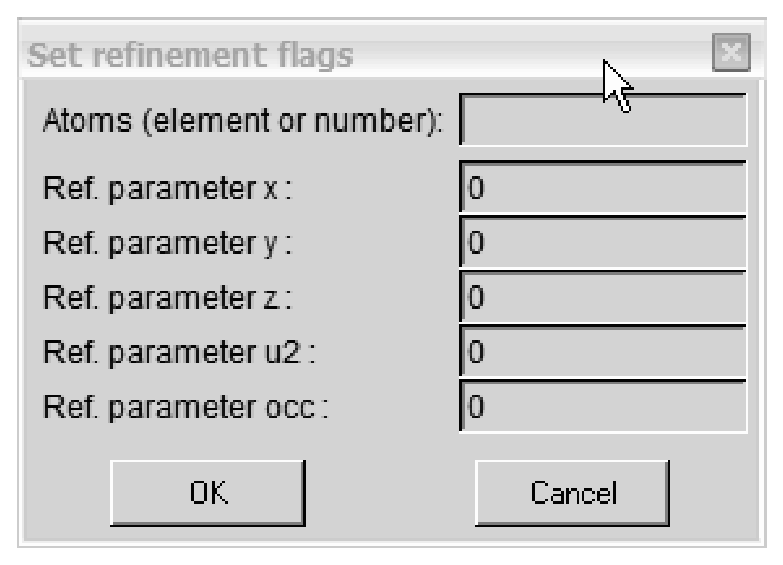
\includegraphics[width=2.0in, angle=0]{use-3.eps}
   \caption{Structural refinement parameters dialog.}
   \label{fig_use3}
\end{figure}

The bottom section of the structural input area contains information
about each atom in the structure. For each atom the following
information is specified: Running index, the element name,
fractional coordinates $x,y,z$ ({\tt x[i],y[i]} and {\tt z[i]}),
position refinement parameters, atomic displacement parameter
$\rangle u^2 \langle$ ({\tt u[i,j]}) with its refinement parameters
and finally the occupancy ({\tt o[i]}) followed by its refinement
parameter. Although {\it PDFFIT} is capable to refine anisotropic
atomic displacement parameters, this feature is currently not
implemented in {\it PDFFIT Gui}. In cases where anisotropic atomic
displacement parameters are required, {\it PDFFIT} must be run
without the graphical interface. The header line contains several
buttons: \textbf{Number} allows one to specify the number of atoms
in the structure. Clicking on \textbf{Ref.} bring up the dialog box
shown in Figure \ref{fig_use3}. This dialog allows one to set
refinement parameters for a group of atoms. The atoms can be
specified via their name or number. For example {\tt Ni,2,5-10}
would set the entered refinement parameters for all Ni atoms, atom
number 2 and atoms 5 through 10. Details about the parameter coding
for atom positions and how to implement symmetry constraints are
discussed in section \ref{par}.

%------------------------------------------------------------------------
\section{Data window}

\begin{figure}[!t]
   \centering
   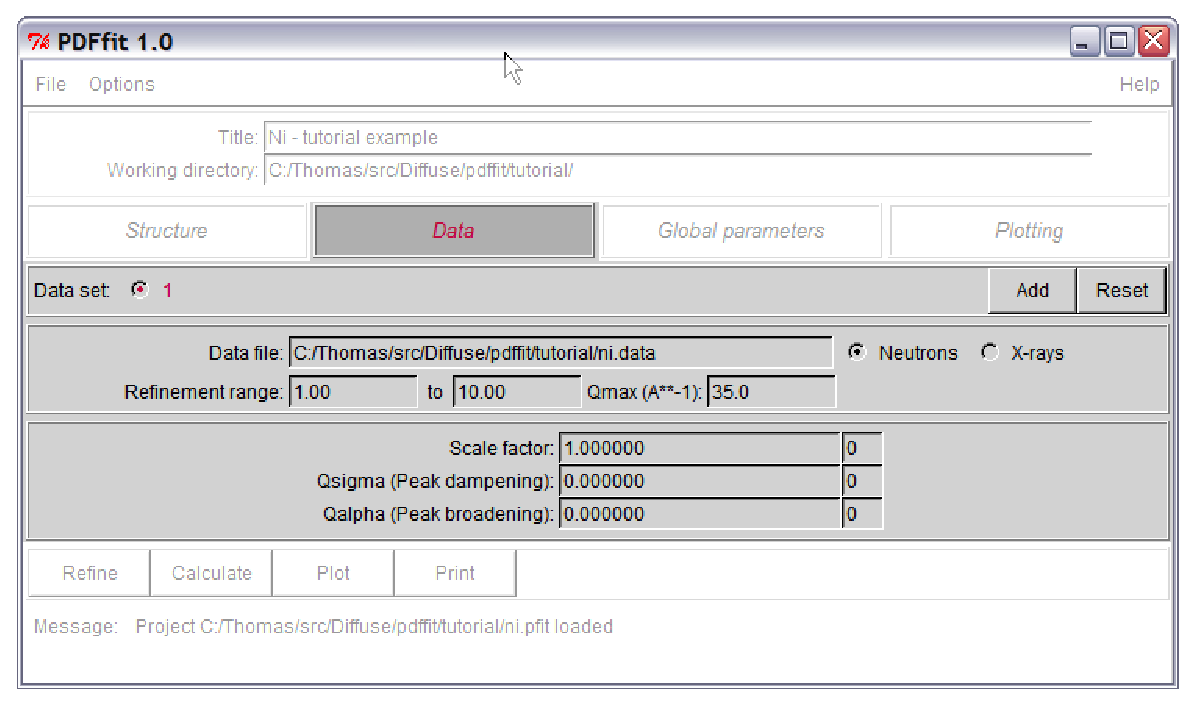
\includegraphics[width=3.5in, angle=0]{use-4.eps}
   \caption{Data window of {\it PDFFIT Gui}.}
   \label{fig_use4}
\end{figure}

The input screen shown in Figure \ref{fig_use4} appears when the
{\bf Data} button is pressed. All information related to the
experimental PDF data sets is entered here. Similar to the selection
of multiple phases in the structure window, the program allows to
refine multiple data sets. The top left radio buttons select the
data set and the button on the right allow one to add a data set
({\bf Add}) or reset the number of data sets to one ({\bf Reset}).
\par

The area underneath contains a field for the data file name. By
right clicking in this field, the data set can be selected using a
file dialog box. The data file needs to be a valid {\it PDFFIT} data
file. For details about the file formats, refer to the {\it PDFFIT}
users guide. The other fields allow to select the data set type,
either neutron or x-ray data. The refinement range is specified
below. It determines not only the range in $r$ used in the
refinement, but also the calculation range for the PDF when the
button {\bf Calculate} is pressed. The final input in this art is
the value $Q_{max}$ used to terminate the diffraction data. If a
data file produced by {\it PDFgetN} is read, this value is
automatically set based on the information in the data file. \par

The next section down contains all data set specific parameters
related to the current data set. Again, the small input fields just
right of the value entry field allows one to specify a refinement
parameter. The parameters are

\begin{itemize}
  \item \textbf{Scale factor}: This specifies the scale factor for the
  selected data set. ({\it PDFFIT}: {\tt dsca[s]})

  \item \textbf{Qsigma}: This specifies the resolution dampening, $\sigma_Q$
  for the selected data set. ({\it PDFFIT}: {\tt qsig[s]})

  \item \textbf{Qalpha}: This specifies the resolution broadening, $\alpha$
  for the selected data set. ({\it PDFFIT}: {\tt qalp[s]})
\end{itemize}

%------------------------------------------------------------------------
\section{Global parameters window}

\begin{figure}[!t]
   \centering
   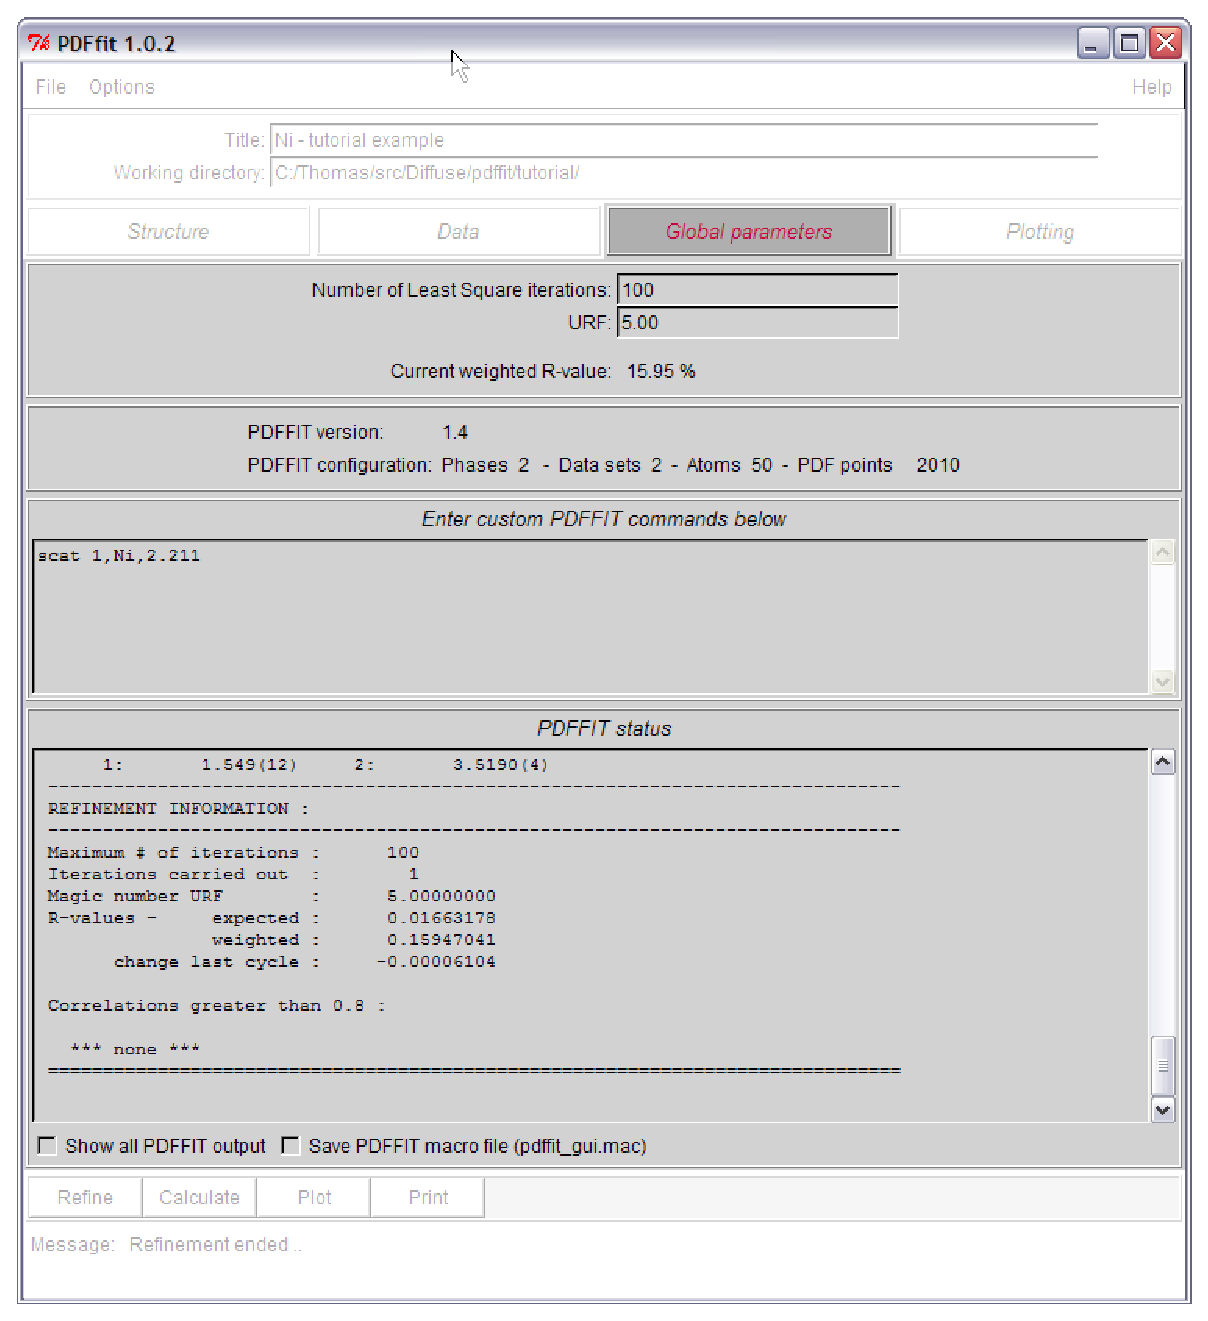
\includegraphics[width=3.5in, angle=0]{use-5.eps}
   \caption{Generic window of {\it PDFFIT Gui}.}
   \label{fig_use5}
\end{figure}

Clicking the button {\bf Global parameters} will show the input
screen related to general refinement settings as well as showing the
output of {\it PDFFIT}. The two top most fields specify the maximum
number of refinement iterations as well as the URF value. The URF
value determines the 'refinement speed' and is discussed in the {\it
PDFFIT} users guide. Next the weighted R-value of the last
refinement of PDF calculation is shown. The frame below contains
information about the version as well as configuration of the {it
PDFFIT} program running. If configuration settings such as the
maximum number of atoms need to be changed, the program {\it PDFFIT}
needs to be re-compiled. Instructions how to do this can be found in
the {\it PDFFIT} users guide. \par

The center frame allows one to specify arbitrary {\it PDFFIT}
commands, that are executed just before the refinement or
calculation command. For details about {\it PDFFIT} commands, please
refer to the {\it PDFFIT} users guide.

The next frame down contains commands and output of the program {\it
PDFFIT} during the last refinement or calculation. A scrollbar
allows one to browse through the output. At the end of a refinement,
the results are shown. A checkbox just below this output area allows
one to force {\it PDFFIT Gui} to show {\it all} commands and output
of the {\it PDFFIT} program. Note, that depending on the operating
system and computer speed, the update of the refinement output might
be intermittent. If the second checkbox is checked, the macro file
that is passed to {\it PDFFIT} is saved to the file {\tt
pdffit\_gui.mac} in the current working directory. This macro file
can be used and modified for refinements outside of this graphical
interface.

%------------------------------------------------------------------------
\section{Plotting}

\begin{figure}[!t]
   \centering
   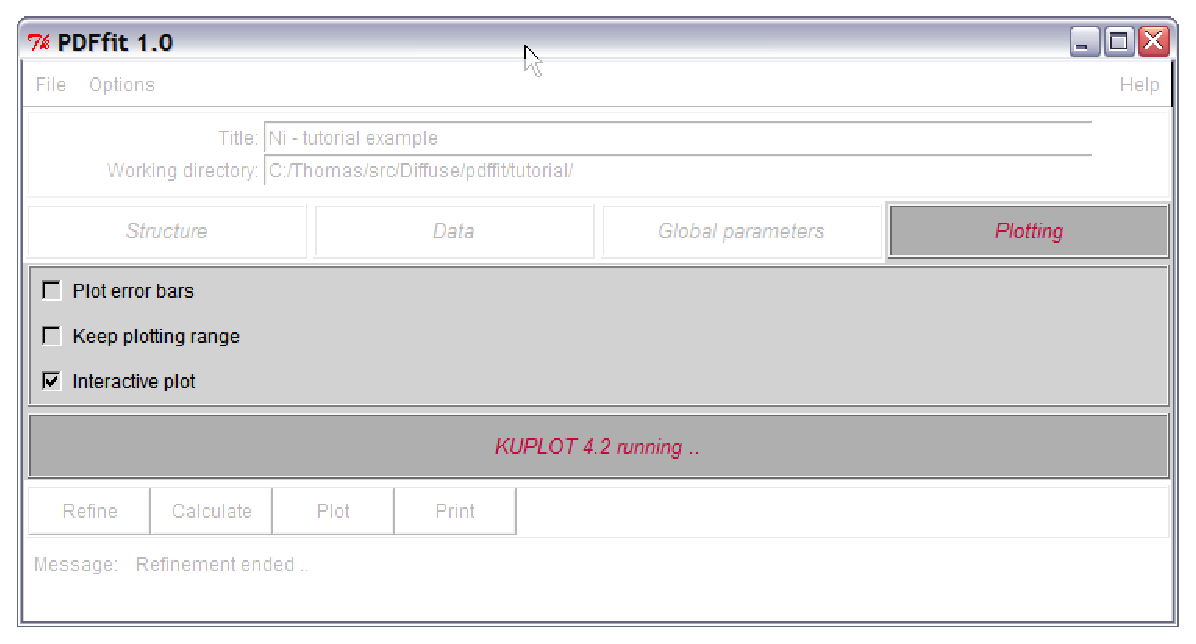
\includegraphics[width=3.5in, angle=0]{use-6.eps}
   \caption{Plotting parameter window of {\it PDFFIT Gui}.}
   \label{fig_use6}
\end{figure}

\begin{figure}[!t]
   \centering
   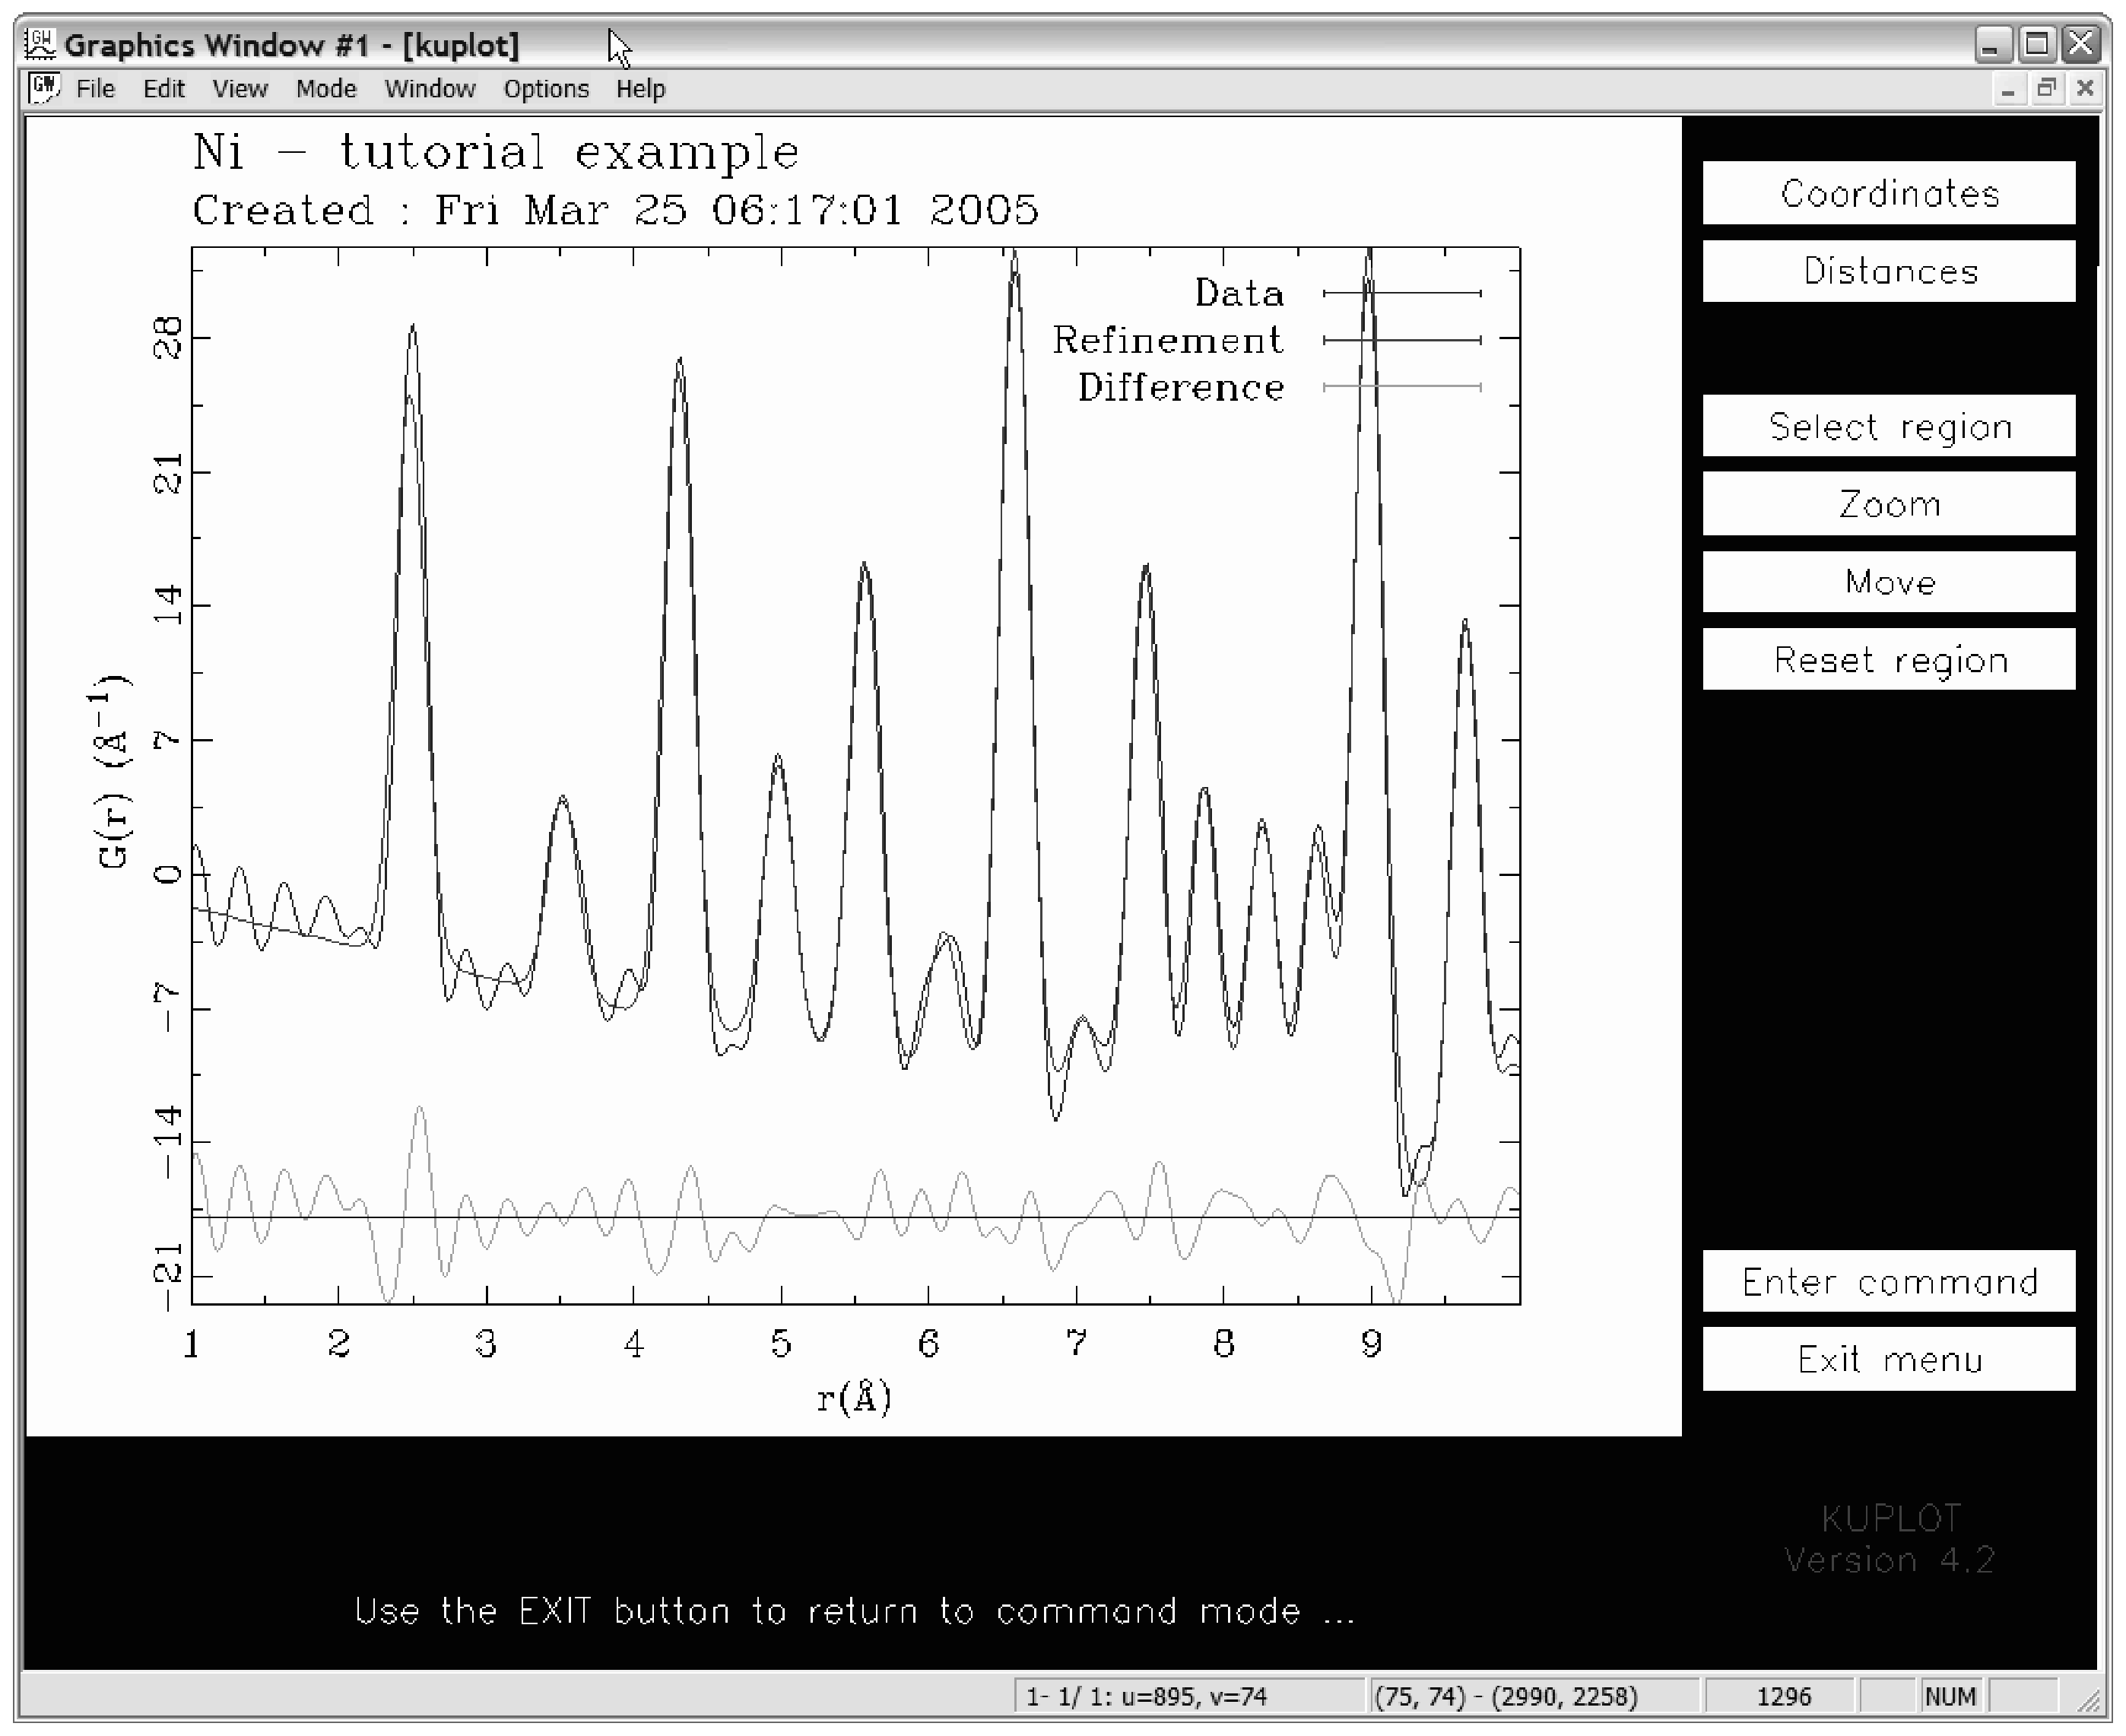
\includegraphics[width=3.5in, angle=0]{use-7.eps}
   \caption{Plotting output of {\it PDFFIT Gui}.}
   \label{fig_use7}
\end{figure}

Clicking the button {\bf Plotting} will show the input screen
containing all plotting options. Note that {\it KUPLOT} must be
installed for the plotting option to work. If {\it KUPLOT} is not
found, this screen will simply show {\tt No KUPLOT found}. The line
colors used by {\it KUPLOT} can be changed using the {\tt Options}
menu. The three options on this screen are listed below.

\begin{itemize}
  \item \textbf{Plot error bars}: This will plot error bars for the
  experimental PDF.

  \item \textbf{Keep plotting range}: If this box is checked, the
  selected plotting range used in the previous plot will be kept.
  Otherwise, the plot is scales to show the full refinement range.

  \item \textbf{Interactive plot}: If this box is checked, {\it
  KUPLOT} will show a series of buttons allowing one to interact
  with the plot, e.g. zoom into a specific region. The output plot
  window is shown in Figure \ref{fig_use7}. Note that one needs to
  exit this menu via {\tt Exit menu} before regaining control of the
  main program.
\end{itemize}

%------------------------------------------------------------------------

\section{Refinement parameters \label{par}}

In this section, we will discuss the concept of refinement
parameters. Since the refinement engine is {\it PDFFIT}, we first
need to recall how {\it PDFFIT} works. Every structural parameter in
{\it PDFFIT} has an associated variable, e.g. the lattice parameter
$a$ is {\tt lat[1]}, the position of atom number 1 is {\tt x[1]} and
so on. Each of these variables can be associated with a refinement
parameter {\tt p[i]}. For example the set of {\it PDFFIT} commands
needed to refine the lattice parameters of a cubic crystal is shown
below.

\begin{MacVerbatim}
  par lat[1]=p[1],1.0
  par lat[2]=p[1],1.0
  par lat[3]=p[1],1.0
\end{MacVerbatim}

This causes all three lattice parameters, $a,b$ and $c$ to be
refined using the {\it same} refinement parameter {\tt p[1]}. This
way one can introduce constraints by using the same refinement
parameter several times. In {\it PDFFIT} itself, one can use more
complex constraint equations. In this graphical interface, one
simple specifies the parameter number to be used in the field
associated with the desired variable. Constraints are implemented
the same way by simply specifying the same parameter number for all
variables that are required to have the same value. Obviously, one
needs to take care not to use a refinement parameter value twice
unintentionally.\par

In order to allow symmetry constraints to be implemented straight
forwardly, the use of the refinement parameter number for atom
positions, $x, y$ and $z$, is different. In this case the parameter
is not refining the value itself, but an offset. A negative number
causes the offset to be subtracted whereas a positive number will
add the offset. Let us assume we had an atom at $x,y,z$ and a
symmetrically equivalent one at $\overline{x},y,\overline{z}+0.5$.
The goal is to refine the positions of both atoms sing just three
refinement parameters and keeping the symmetry relationship. For the
first atom we would specify refinement parameter values 1,2,3 (or
any other three numbers). For the second atom, we need to specify
-1,2,-3, because for $x$ and $y$ the offset needs to be applied in
the opposite direction with respect to the first atom.

%------------------------------------------------------------------------

\section{Output files}

The program {\it PDFFIT Gui} generates several intermediate files
called {\tt pdffit\_work*} while running. These files, however, are
deleted once one exits the program. In order to save the current
settings and refinement results, choose {\tt Save} from the {\tt
File} menu. This will save the following files in the specified
directory

\begin{itemize}
  \item {\tt file.pfit}: This text file contains all the setting of
  {\it PDFFIT Gui} for the current project. On the Windows
  operating system, this file extension is associated with {\it
  PDFFIT Gui} and by double clicking on such as file, {\it PDFFIT
  Gui} will be launched and the file read. Alternatively one can
  load such a file using the {\tt File - Load} menu.

  \item {\tt file.res}: This is the result file produced by {\it
  PDFFIT}.

  \item {\tt file\_pX.rstr}: This is the resulting structure file for
  phase $X$ in {\it PDFFIT} format.

  \item {\tt file\_dX.calc} and {\tt file\_dX.dif}: These are the
  calculated PDF and the difference between calculated and
  experimental PDF for data set $X$, respectively.
\end{itemize}


%------------------------------------------------------------------------
